\documentclass{article}%
\usepackage[T1]{fontenc}%
\usepackage[utf8]{inputenc}%
\usepackage{lmodern}%
\usepackage{textcomp}%
\usepackage{lastpage}%
\usepackage[head=40pt,margin=0.5in,bottom=0.6in]{geometry}%
\usepackage{graphicx}%
%
\title{\textbf{Protestaron en Táchira contra el gobierno de Nicolás Maduro}}%
\author{El Nacional Web}%
\date{10/10/2018}%
%
\begin{document}%
\normalsize%
\maketitle%
\textbf{URL: }%
http://www.el{-}nacional.com/noticias/protestas/protestaron{-}tachira{-}contra{-}gobierno{-}nicolas{-}maduro\_255204\newline%
%
\textbf{Periodico: }%
EN, %
ID: %
255204, %
Seccion: %
Protestas\newline%
%
\textbf{Palabras Claves: }%
Táchira, Protestas, Sociedad\newline%
%
\textbf{Derecho: }%
2.3, %
Otros Derechos: %
2.8, %
Sub Derechos: %
2.3.4, 2.8.1\newline%
%
\textbf{EP: }%
SI\newline%
\newline%
%
\textbf{\textit{Los ciudadanos criticaron las condiciones en las que se encuentran los entes públicos y privados del país}}%
\newline%
\newline%
%
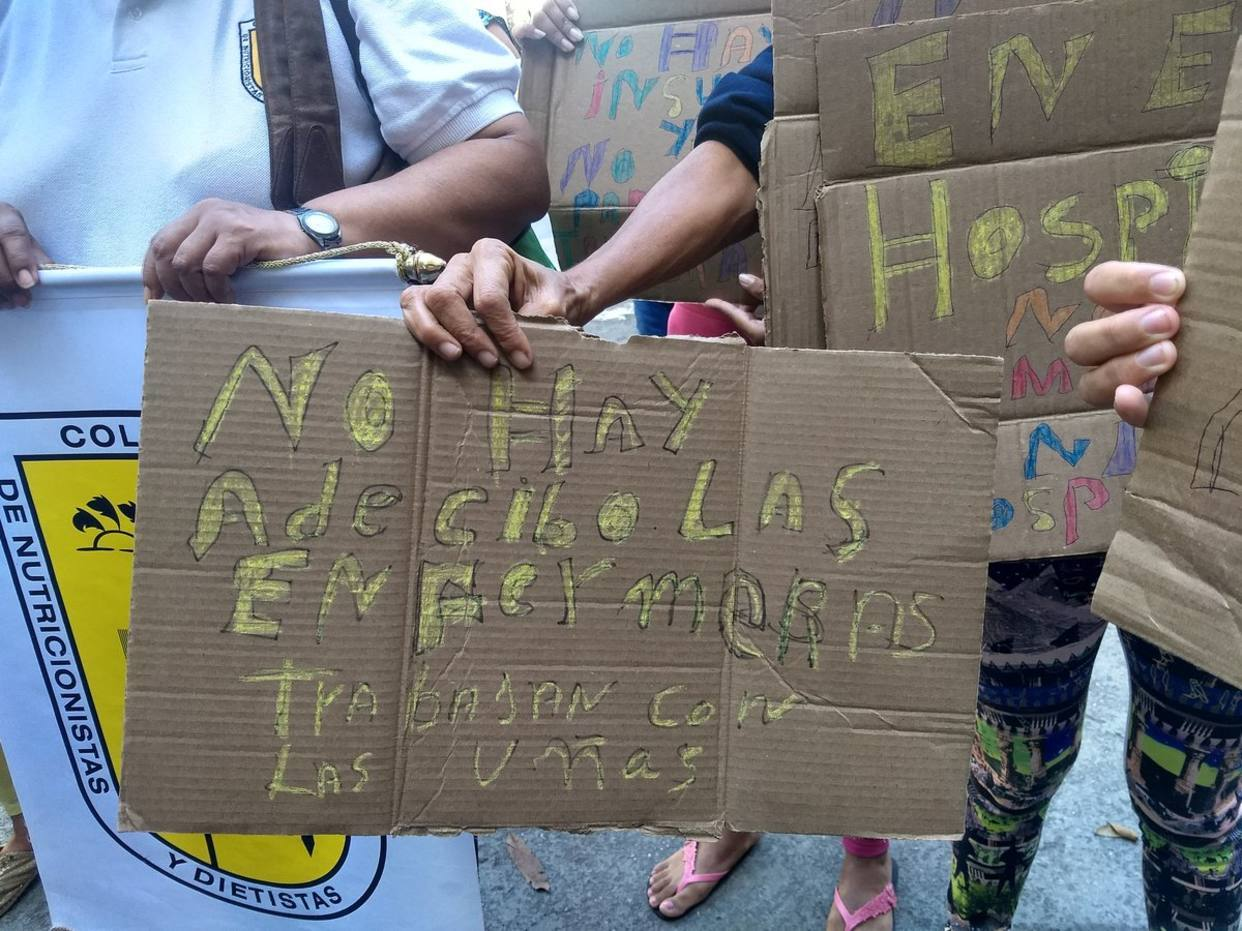
\includegraphics[width=300px]{167.jpg}%
\newline%
%
Este miércoles en horas del mediodía trabajadores de la salud, de la Universidad de los Andes (ULA) y de la Universidad Nacional Experimental del Táchira (UNET), protestaron contra el gobierno de Nicolás Maduro.%
\newline%
%
La periodista Lorena Bornacelly indicó que los ciudadanos de Táchira también criticaron las condiciones en las que se encuentran los entes públicos y privados del país.%
\newline%
%
“Mi única arma es mi voz”, se pudo~leer en uno de los carteles que sostuvieron~durante la protesta.%
\newline%
%
\end{document}